\let\negmedspace\undefined
\let\negthickspace\undefined
\documentclass[journal]{IEEEtran}
\usepackage[a5paper, margin=10mm, onecolumn]{geometry}
%\usepackage{lmodern} % Ensure lmodern is loaded for pdflatex
\usepackage{tfrupee} % Include tfrupee package
\setlength{\headheight}{1cm} % Set the height of the header box
\setlength{\headsep}{0mm}     % Set the distance between the header box and the top of the text
\usepackage{gvv-book}
\usepackage{gvv}
\usepackage{cite}
\usepackage{amsmath,amssymb,amsfonts,amsthm}
\usepackage{algorithmic}
\usepackage{graphicx}
\usepackage{textcomp}
\usepackage{xcolor}
\usepackage{txfonts}
\usepackage{listings}
\usepackage{enumitem}
\usepackage{mathtools}
\usepackage{gensymb}
\usepackage{comment}
\usepackage[breaklinks=true]{hyperref}
\usepackage{tkz-euclide} 
\usepackage{listings}
% \usepackage{gvv}                                        
\def\inputGnumericTable{}                                 
\usepackage[latin1]{inputenc}                                
\usepackage{color}                                            
\usepackage{array}                                            
\usepackage{longtable}                                       
\usepackage{calc}                                             
\usepackage{multirow}                                         
\usepackage{hhline}                                           
\usepackage{ifthen}                                           
\usepackage{lscape}
\begin{document}

\bibliographystyle{IEEEtran}
\vspace{3cm}
\parindent 0px

\title{9.4.21}
\author{EE24BTECH11050 - Pothuri Rahul}
% \maketitle
% \newpage
% \bigskip
{\let\newpage\relax\maketitle}

\renewcommand{\thefigure}{\theenumi}
\renewcommand{\thetable}{\theenumi}
\setlength{\intextsep}{10pt} % Space between text and floats


\numberwithin{equation}{enumi}
\numberwithin{figure}{enumi}
\renewcommand{\thetable}{\theenumi}

\textbf{Question:} \\
In a bank,principal increases continuously at the rate of $5\%$ per year. An amount of rupees $1000$ is deposited with this bank. How much will it worth after 10 years $\brak{e^{0.5} = 1.648}$ \\ \\
\solution 
\begin{table}[h!]
    \centering
    \begin{tabular}{|l|l|l|}
\hline
\textbf{Component} & \textbf{Arduino Pin} & \textbf{Description} \\
\hline
\multicolumn{3}{|c|}{\textbf{LCD Display}} \\
\hline
RS & PB0 (Digital 8) & Register Select line \\
\hline
E & PB1 (Digital 9) & Enable line \\
\hline
D4 & PB2 (Digital 10) & Data line 4 \\
\hline
D5 & PB3 (Digital 11) & Data line 5 \\
\hline
D6 & PB4 (Digital 12) & Data line 6 \\
\hline
D7 & PB5 (Digital 13) & Data line 7 \\
\hline
\multicolumn{3}{|c|}{\textbf{7-Segment Display}} \\
\hline
Segment A & PD4 (Digital 4) & Segment A line \\
\hline
Segment B & PD5 (Digital 5) & Segment B line \\
\hline
Segment C & PD6 (Digital 6) & Segment C line \\
\hline
Segment D & PD7 (Digital 7) & Segment D line \\
\hline
Common HH\_1 & PC0 (Analog 0) & Hours tens digit common \\
\hline
Common HH\_2 & PC1 (Analog 1) & Hours ones digit common \\
\hline
Common MM\_1 & PC2 (Analog 2) & Minutes tens digit common \\
\hline
Common MM\_2 & PC3 (Analog 3) & Minutes ones digit common \\
\hline
Common SS\_1 & PC4 (Analog 4) & Seconds tens digit common \\
\hline
Common SS\_2 & PC5 (Analog 5) & Seconds ones digit common \\
\hline
\multicolumn{3}{|c|}{\textbf{Buttons}} \\
\hline
Toggle Button & PD2 (Digital 2) & For cycling through options \\
\hline
Select Button & PD3 (Digital 3) & For selecting options \\
\hline
\end{tabular}
    \caption{Variables Used}
    
\end{table}
\\
\solution Let P be the principle at any time t. According to the given problem, Rate of change in principle can be given as 
\begin{align}
\frac{dP}{dt} = \brak{\frac{5}{100}} \times P \label{1}
\end{align}
\begin{align}
\frac{dP}{dt} = \brak{\frac{P}{20}} \label{2}
\end{align}
Seperating the variables in the equation \eqref{2}, We get 
\begin{align}
\frac{dP}{P}=\frac{dt}{20} \label{3}
\end{align}
On integrating both sides
\begin{align}
\int \frac{dP}{P}=\int \frac{dt}{20} \label{4} \\
log P = \frac{t}{20}+C \label{5} \\
P=e^{\frac{t}{20}+C} \label{6} \\
P=e^{\frac{t}{20}} . e^{C} \label{7} \\
P=e^{\frac{t}{20}} . C_1 \label{8}
\end{align}
Given, at time t=0,$P_0$=1000 then, from \eqref{8}
\begin{align}
1000=C_1 \label{9}
\end{align}
Principle can be given as 
\begin{align}
P = 1000 \times e^{\frac{t}{20}} \label{10}
\end{align}
At time t=10,Principle can be given as \\
\begin{align}
P =1000 \times e^{\frac{10}{20}} \\
P =1000 \times e^{0.5} \\
P = 1000 \times 1.648 \\
P = 1648
\end{align}
\textbf{Logic used for programming:-} \\
\textbf{Method of finite differences:} This method is used to find the approximate solution of the given differential equation by using the values of the function at discrete points.  \\
From the defination of derivative of a function 
\begin{align}
\frac{dy}{dx} \approx \frac{y\brak{x+h}-y\brak{x}}{h} \label{11}
\end{align}
by rearranging the terms, we get the function
\begin{align}
y\brak{x+h}=y\brak{x}+h \times \frac{dy}{dx} \\
P\brak{t+h}=P\brak{t}+h \times \frac{P}{20}
\end{align}
Let \brak{t_0,P_0} be points on the curve,
\begin{align}
t_1=t_0+h \\
P_1=P_0+h \times \frac{P}{20}
\end{align}
On  generalising the above equations,
\begin{align}
t_{n+1}=t_{n}+h \\
P_{n+1}=P_{n}+h \times \frac{P}{20} \label{21}
\end{align}
Where h is a very small division (example 0.1),We need iterate this algorithm by taking $P_0=1000$ and $t=0$, till $t_n=10$. Then we get the principle amount after 10 years.
If we plot all the points $(t,P)$, we get the function P varying with t, i.e P vs T graph. \\

\textbf{Finding the solution of this equation using the Z-Transform:} By using the z-transform method we can convert the differential equation into a linear equation in Z-domain,after finding the solution in z-domin,inverse of it is the solution of the given differential equation. \\
The differential equation for this question is,
\begin{align}
\frac{dP}{dt}=\frac{P}{20}
\end{align}
from \eqref{21}, \\
\begin{align}
P_{n+1}=P_{n}+h \times \frac{P_n}{20} \\
P_{n+1}=P_{n}(1+\frac{h}{20})
\end{align}
Applying Z-tranform on both sides,We get,
\begin{align}
Z\brak{P_{n+1}}=Z\brak{P_{n}(1+\frac{h}{20})} \\
Z(P_n+1)=(1+\frac{h}{20})Z(P_n)
\end{align}
Let,
\begin{align}
Z\brak{P_n}=P\brak{z}
\end{align}
Then,
\begin{align}
Z\brak{P_{n+1}}=zP(z)-zP_0
\end{align}
Now,
\begin{align}
zP(z)-zP_0 = P(z)(1+h/20) \\
P(z) \sbrak{z-\brak{1+\frac{h}{20}}} = zP_0 \\
\end{align}
\begin{align}
P(z) = P_0 \sbrak{\frac{z}{z-\brak{1+\frac{h}{20}}}}
\end{align}
By inversing, we get 
\begin{align}
P_n = P_0 \times \brak{1+\frac{h}{20}}^n
\end{align}
We know that,
\begin{align}
1+\frac{h}{20} \approx e^{\frac{h}{20}}
\end{align}
then,
\begin{align}
P_n = P_0 \brak{e^{\frac{h}{20}}}^n \\
P_n = P_o e^{\frac{nh}{20}}
\end{align}
As h is the small division of time and n are the total no.of divisions, nh turns to be t at that point,Then
\begin{align}
P\brak{t}=P_0e^{\frac{t}{20}}
\end{align}



\begin{figure}[htbp] % Positioning options: here, top, bottom, page
    \centering
    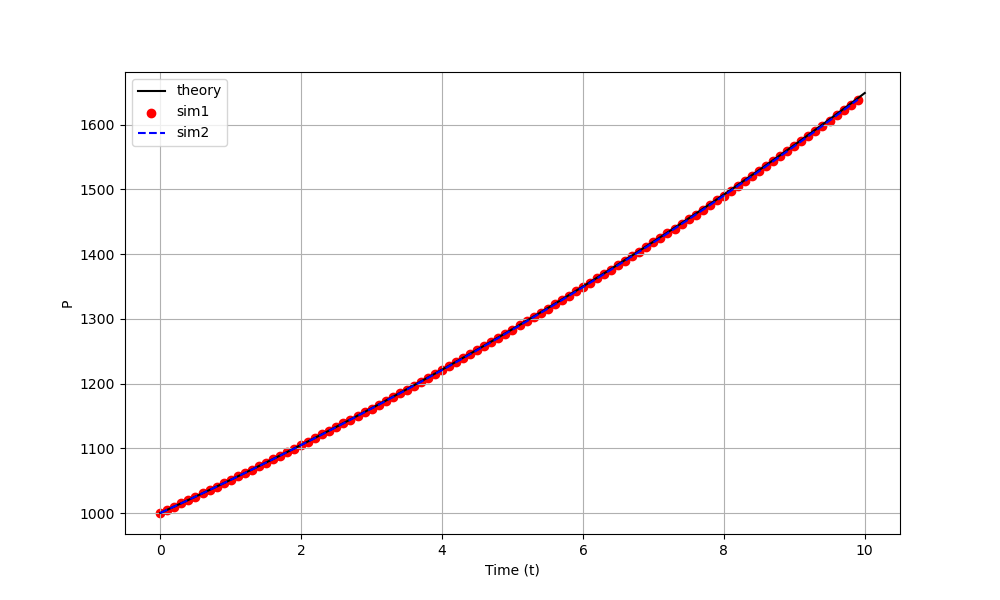
\includegraphics[width=\textwidth]{fig/plot.png} % Replace "filename" with your image file
    \caption{Plot}
\end{figure}



\end{document}
